\documentclass[14pt]{extbook}
\usepackage{multicol, enumerate, enumitem, hyperref, color, soul, setspace, parskip, fancyhdr} %General Packages
\usepackage{amssymb, amsthm, amsmath, latexsym, units, mathtools} %Math Packages
\everymath{\displaystyle} %All math in Display Style
% Packages with additional options
\usepackage[headsep=0.5cm,headheight=12pt, left=1 in,right= 1 in,top= 1 in,bottom= 1 in]{geometry}
\usepackage[usenames,dvipsnames]{xcolor}
\usepackage{dashrule}  % Package to use the command below to create lines between items
\newcommand{\litem}[1]{\item#1\hspace*{-1cm}\rule{\textwidth}{0.4pt}}
\pagestyle{fancy}
\lhead{Progress Quiz 8}
\chead{}
\rhead{Version ALL}
\lfoot{5493-4176}
\cfoot{}
\rfoot{Summer C 2021}
\begin{document}

\begin{enumerate}
\litem{
First, find the equation of the line containing the two points below. Then, write the equation in the form $ y=mx+b $ and choose the intervals that contain $m$ and $b$.\[ (3, 8) \text{ and } (4, 2) \]\begin{enumerate}[label=\Alph*.]
\item \( m \in [-11, -5] \hspace*{3mm} b \in [26, 27] \)
\item \( m \in [3, 9] \hspace*{3mm} b \in [-24, -21] \)
\item \( m \in [-11, -5] \hspace*{3mm} b \in [-10, -1] \)
\item \( m \in [-11, -5] \hspace*{3mm} b \in [-26, -23] \)
\item \( m \in [-11, -5] \hspace*{3mm} b \in [4, 8] \)

\end{enumerate} }
\litem{
Solve the equation below. Then, choose the interval that contains the solution.\[ -14(2x -19) = -10(17x -16) \]\begin{enumerate}[label=\Alph*.]
\item \( x \in [-3.01, -2.31] \)
\item \( x \in [2.85, 3.54] \)
\item \( x \in [2.03, 2.61] \)
\item \( x \in [-0.76, -0.56] \)
\item \( \text{There are no real solutions.} \)

\end{enumerate} }
\litem{
Write the equation of the line in the graph below in Standard Form $Ax+By=C$. Then, choose the intervals that contain $A, B, \text{ and } C$.
\begin{center}
    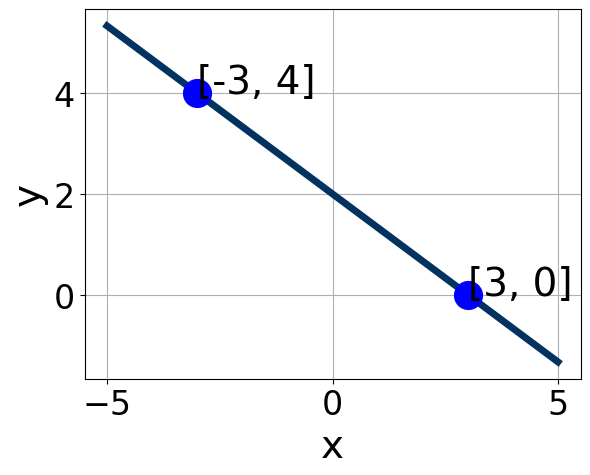
\includegraphics[width=0.5\textwidth]{../Figures/linearGraphToStandardA.png}
\end{center}
\begin{enumerate}[label=\Alph*.]
\item \( A \in [1.75, 2.91], \hspace{3mm} B \in [-3.69, -2.65], \text{ and } \hspace{3mm} C \in [-6.6, -2.8] \)
\item \( A \in [0.41, 1.52], \hspace{3mm} B \in [0.76, 1.89], \text{ and } \hspace{3mm} C \in [1, 3.1] \)
\item \( A \in [0.41, 1.52], \hspace{3mm} B \in [-1.97, -0.93], \text{ and } \hspace{3mm} C \in [-3.9, 0.2] \)
\item \( A \in [1.75, 2.91], \hspace{3mm} B \in [2.11, 4.64], \text{ and } \hspace{3mm} C \in [5.6, 7.5] \)
\item \( A \in [-2.7, -0.81], \hspace{3mm} B \in [-3.69, -2.65], \text{ and } \hspace{3mm} C \in [-6.6, -2.8] \)

\end{enumerate} }
\litem{
Find the equation of the line described below. Write the linear equation in the form $ y=mx+b $ and choose the intervals that contain $m$ and $b$.\[ \text{Parallel to } 8 x - 5 y = 12 \text{ and passing through the point } (-6, -5). \]\begin{enumerate}[label=\Alph*.]
\item \( m \in [1.37, 1.62] \hspace*{3mm} b \in [-7.6, -3.6] \)
\item \( m \in [0.41, 0.7] \hspace*{3mm} b \in [2.6, 5.6] \)
\item \( m \in [-1.74, -0.49] \hspace*{3mm} b \in [-18.6, -11.6] \)
\item \( m \in [1.37, 1.62] \hspace*{3mm} b \in [0, 2] \)
\item \( m \in [1.37, 1.62] \hspace*{3mm} b \in [2.6, 5.6] \)

\end{enumerate} }
\litem{
Solve the linear equation below. Then, choose the interval that contains the solution.\[ \frac{-7x + 4}{3} - \frac{-6x -5}{2} = \frac{5x + 7}{5} \]\begin{enumerate}[label=\Alph*.]
\item \( x \in [4.5, 6.5] \)
\item \( x \in [-9.6, -6.7] \)
\item \( x \in [-1.4, 1.5] \)
\item \( x \in [6.6, 7.6] \)
\item \( \text{There are no real solutions.} \)

\end{enumerate} }
\litem{
Find the equation of the line described below. Write the linear equation in the form $ y=mx+b $ and choose the intervals that contain $m$ and $b$.\[ \text{Parallel to } 4 x - 7 y = 14 \text{ and passing through the point } (-8, -6). \]\begin{enumerate}[label=\Alph*.]
\item \( m \in [-0.02, 0.95] \hspace*{3mm} b \in [1.67, 2.54] \)
\item \( m \in [1.64, 2.32] \hspace*{3mm} b \in [-1.62, -1.29] \)
\item \( m \in [-0.02, 0.95] \hspace*{3mm} b \in [-0.04, 1.6] \)
\item \( m \in [-0.02, 0.95] \hspace*{3mm} b \in [-1.62, -1.29] \)
\item \( m \in [-1.06, 0.39] \hspace*{3mm} b \in [-11.81, -8.98] \)

\end{enumerate} }
\litem{
Solve the equation below. Then, choose the interval that contains the solution.\[ -17(-16x -3) = -14(-7x -4) \]\begin{enumerate}[label=\Alph*.]
\item \( x \in [-0.22, 0.15] \)
\item \( x \in [-0.33, -0.2] \)
\item \( x \in [-0.79, -0.61] \)
\item \( x \in [0.34, 0.76] \)
\item \( \text{There are no real solutions.} \)

\end{enumerate} }
\litem{
First, find the equation of the line containing the two points below. Then, write the equation in the form $ y=mx+b $ and choose the intervals that contain $m$ and $b$.\[ (-9, 6) \text{ and } (-5, -4) \]\begin{enumerate}[label=\Alph*.]
\item \( m \in [1.5, 5.5] \hspace*{3mm} b \in [8.2, 9.8] \)
\item \( m \in [-6.5, -1.5] \hspace*{3mm} b \in [0.9, 1.2] \)
\item \( m \in [-6.5, -1.5] \hspace*{3mm} b \in [-18.8, -14.7] \)
\item \( m \in [-6.5, -1.5] \hspace*{3mm} b \in [16, 16.9] \)
\item \( m \in [-6.5, -1.5] \hspace*{3mm} b \in [13.6, 15.9] \)

\end{enumerate} }
\litem{
Write the equation of the line in the graph below in Standard Form $Ax+By=C$. Then, choose the intervals that contain $A, B, \text{ and } C$.
\begin{center}
    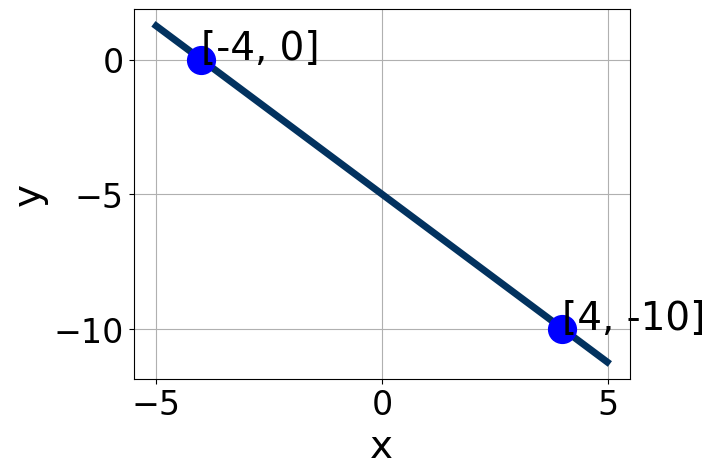
\includegraphics[width=0.5\textwidth]{../Figures/linearGraphToStandardCopyA.png}
\end{center}
\begin{enumerate}[label=\Alph*.]
\item \( A \in [-1.3, 3.1], \hspace{3mm} B \in [-0.06, 1.87], \text{ and } \hspace{3mm} C \in [-6, 1] \)
\item \( A \in [-1.3, 3.1], \hspace{3mm} B \in [-1.57, -0.25], \text{ and } \hspace{3mm} C \in [4, 6] \)
\item \( A \in [3.1, 8.7], \hspace{3mm} B \in [3.44, 4.03], \text{ and } \hspace{3mm} C \in [-21, -19] \)
\item \( A \in [-5.6, -4.8], \hspace{3mm} B \in [-4.51, -2.73], \text{ and } \hspace{3mm} C \in [12, 24] \)
\item \( A \in [3.1, 8.7], \hspace{3mm} B \in [-4.51, -2.73], \text{ and } \hspace{3mm} C \in [12, 24] \)

\end{enumerate} }
\litem{
Solve the linear equation below. Then, choose the interval that contains the solution.\[ \frac{4x + 6}{3} - \frac{4x + 6}{7} = \frac{3x + 4}{8} \]\begin{enumerate}[label=\Alph*.]
\item \( x \in [-2.8, -1.6] \)
\item \( x \in [9.8, 10.6] \)
\item \( x \in [-6.2, -5.6] \)
\item \( x \in [-0.1, 2] \)
\item \( \text{There are no real solutions.} \)

\end{enumerate} }
\litem{
First, find the equation of the line containing the two points below. Then, write the equation in the form $ y=mx+b $ and choose the intervals that contain $m$ and $b$.\[ (6, -7) \text{ and } (11, 6) \]\begin{enumerate}[label=\Alph*.]
\item \( m \in [-8.6, -1.6] \hspace*{3mm} b \in [33.6, 36.6] \)
\item \( m \in [-0.4, 6.6] \hspace*{3mm} b \in [18.6, 28.6] \)
\item \( m \in [-0.4, 6.6] \hspace*{3mm} b \in [-22.6, -20.6] \)
\item \( m \in [-0.4, 6.6] \hspace*{3mm} b \in [-11, -3] \)
\item \( m \in [-0.4, 6.6] \hspace*{3mm} b \in [-15, -11] \)

\end{enumerate} }
\litem{
Solve the equation below. Then, choose the interval that contains the solution.\[ -12(-14x + 17) = -4(-19x + 2) \]\begin{enumerate}[label=\Alph*.]
\item \( x \in [1.94, 2.27] \)
\item \( x \in [2.17, 2.43] \)
\item \( x \in [-2.67, -2.23] \)
\item \( x \in [0.78, 1.12] \)
\item \( \text{There are no real solutions.} \)

\end{enumerate} }
\litem{
Write the equation of the line in the graph below in Standard Form $Ax+By=C$. Then, choose the intervals that contain $A, B, \text{ and } C$.
\begin{center}
    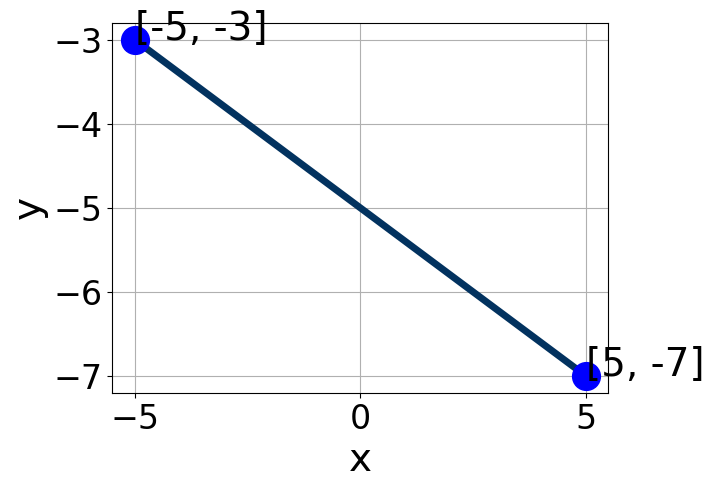
\includegraphics[width=0.5\textwidth]{../Figures/linearGraphToStandardB.png}
\end{center}
\begin{enumerate}[label=\Alph*.]
\item \( A \in [0.1, 1.5], \hspace{3mm} B \in [0.6, 1.8], \text{ and } \hspace{3mm} C \in [-10, -1] \)
\item \( A \in [0.1, 1.5], \hspace{3mm} B \in [-1.4, 0.1], \text{ and } \hspace{3mm} C \in [3, 7] \)
\item \( A \in [1.1, 4.4], \hspace{3mm} B \in [3.4, 7.4], \text{ and } \hspace{3mm} C \in [-26, -24] \)
\item \( A \in [-2.2, -0.9], \hspace{3mm} B \in [-6.1, -4.8], \text{ and } \hspace{3mm} C \in [20, 32] \)
\item \( A \in [1.1, 4.4], \hspace{3mm} B \in [-6.1, -4.8], \text{ and } \hspace{3mm} C \in [20, 32] \)

\end{enumerate} }
\litem{
Find the equation of the line described below. Write the linear equation in the form $ y=mx+b $ and choose the intervals that contain $m$ and $b$.\[ \text{Parallel to } 6 x - 7 y = 13 \text{ and passing through the point } (2, -5). \]\begin{enumerate}[label=\Alph*.]
\item \( m \in [1.13, 2.36] \hspace*{3mm} b \in [-6.84, -4.95] \)
\item \( m \in [-0.01, 1.02] \hspace*{3mm} b \in [-6.84, -4.95] \)
\item \( m \in [-0.01, 1.02] \hspace*{3mm} b \in [6.69, 7.89] \)
\item \( m \in [-0.01, 1.02] \hspace*{3mm} b \in [-7.39, -6.76] \)
\item \( m \in [-1.34, -0.72] \hspace*{3mm} b \in [-3.91, -2.08] \)

\end{enumerate} }
\litem{
Solve the linear equation below. Then, choose the interval that contains the solution.\[ \frac{4x -5}{4} - \frac{5x + 5}{3} = \frac{-8x -9}{8} \]\begin{enumerate}[label=\Alph*.]
\item \( x \in [-0.7, 1.1] \)
\item \( x \in [-4.8, -3] \)
\item \( x \in [5.2, 7.6] \)
\item \( x \in [2.8, 4.1] \)
\item \( \text{There are no real solutions.} \)

\end{enumerate} }
\litem{
Find the equation of the line described below. Write the linear equation in the form $ y=mx+b $ and choose the intervals that contain $m$ and $b$.\[ \text{Parallel to } 6 x + 5 y = 7 \text{ and passing through the point } (-3, -10). \]\begin{enumerate}[label=\Alph*.]
\item \( m \in [-1.12, -0.75] \hspace*{3mm} b \in [-14, -12.98] \)
\item \( m \in [-2.5, -0.92] \hspace*{3mm} b \in [13.21, 13.82] \)
\item \( m \in [0.75, 1.71] \hspace*{3mm} b \in [-6.99, -6.29] \)
\item \( m \in [-2.5, -0.92] \hspace*{3mm} b \in [-14, -12.98] \)
\item \( m \in [-2.5, -0.92] \hspace*{3mm} b \in [-7.27, -6.62] \)

\end{enumerate} }
\litem{
Solve the equation below. Then, choose the interval that contains the solution.\[ -18(19x -12) = -13(-15x -14) \]\begin{enumerate}[label=\Alph*.]
\item \( x \in [-0.8, -0.54] \)
\item \( x \in [0.05, 0.16] \)
\item \( x \in [2.66, 2.9] \)
\item \( x \in [0.58, 1.12] \)
\item \( \text{There are no real solutions.} \)

\end{enumerate} }
\litem{
First, find the equation of the line containing the two points below. Then, write the equation in the form $ y=mx+b $ and choose the intervals that contain $m$ and $b$.\[ (9, 5) \text{ and } (10, -5) \]\begin{enumerate}[label=\Alph*.]
\item \( m \in [-12, -6] \hspace*{3mm} b \in [-4, 0] \)
\item \( m \in [-12, -6] \hspace*{3mm} b \in [-95, -91] \)
\item \( m \in [-12, -6] \hspace*{3mm} b \in [93, 103] \)
\item \( m \in [-12, -6] \hspace*{3mm} b \in [-16, -13] \)
\item \( m \in [8, 15] \hspace*{3mm} b \in [-105, -102] \)

\end{enumerate} }
\litem{
Write the equation of the line in the graph below in Standard Form $Ax+By=C$. Then, choose the intervals that contain $A, B, \text{ and } C$.
\begin{center}
    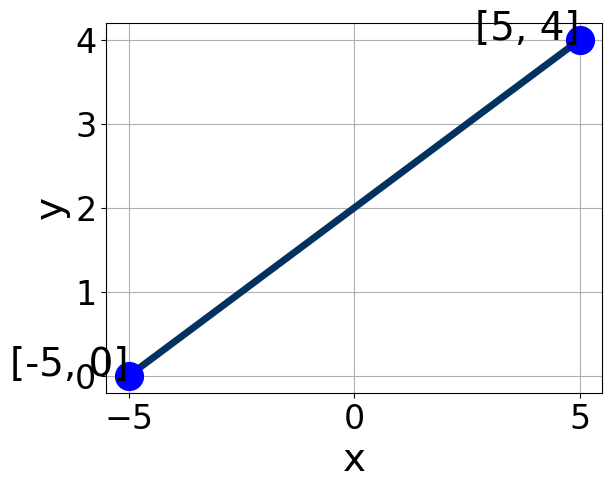
\includegraphics[width=0.5\textwidth]{../Figures/linearGraphToStandardCopyB.png}
\end{center}
\begin{enumerate}[label=\Alph*.]
\item \( A \in [-6.4, -1.5], \hspace{3mm} B \in [1.2, 6.5], \text{ and } \hspace{3mm} C \in [4, 12] \)
\item \( A \in [0.8, 5.6], \hspace{3mm} B \in [-5.3, -3.1], \text{ and } \hspace{3mm} C \in [-15, -5] \)
\item \( A \in [-1.3, -0.3], \hspace{3mm} B \in [-1.7, -0.3], \text{ and } \hspace{3mm} C \in [-8, 1] \)
\item \( A \in [0.8, 5.6], \hspace{3mm} B \in [1.2, 6.5], \text{ and } \hspace{3mm} C \in [4, 12] \)
\item \( A \in [-1.3, -0.3], \hspace{3mm} B \in [0.7, 3.9], \text{ and } \hspace{3mm} C \in [1, 5] \)

\end{enumerate} }
\litem{
Solve the linear equation below. Then, choose the interval that contains the solution.\[ \frac{8x -7}{5} - \frac{5x -3}{4} = \frac{7x + 6}{7} \]\begin{enumerate}[label=\Alph*.]
\item \( x \in [-4.32, -1.32] \)
\item \( x \in [-5.63, -3.63] \)
\item \( x \in [-0.38, 2.62] \)
\item \( x \in [-16.38, -14.38] \)
\item \( \text{There are no real solutions.} \)

\end{enumerate} }
\litem{
First, find the equation of the line containing the two points below. Then, write the equation in the form $ y=mx+b $ and choose the intervals that contain $m$ and $b$.\[ (-5, -7) \text{ and } (-7, 9) \]\begin{enumerate}[label=\Alph*.]
\item \( m \in [-12, -6] \hspace*{3mm} b \in [44, 52] \)
\item \( m \in [-12, -6] \hspace*{3mm} b \in [16, 22] \)
\item \( m \in [-12, -6] \hspace*{3mm} b \in [-52, -46] \)
\item \( m \in [5, 12] \hspace*{3mm} b \in [62, 72] \)
\item \( m \in [-12, -6] \hspace*{3mm} b \in [-6, 6] \)

\end{enumerate} }
\litem{
Solve the equation below. Then, choose the interval that contains the solution.\[ -5(-19x + 6) = -11(14x + 18) \]\begin{enumerate}[label=\Alph*.]
\item \( x \in [-3.99, -3.73] \)
\item \( x \in [0.91, 1.45] \)
\item \( x \in [-0.83, -0.37] \)
\item \( x \in [-1.35, -0.74] \)
\item \( \text{There are no real solutions.} \)

\end{enumerate} }
\litem{
Write the equation of the line in the graph below in Standard Form $Ax+By=C$. Then, choose the intervals that contain $A, B, \text{ and } C$.
\begin{center}
    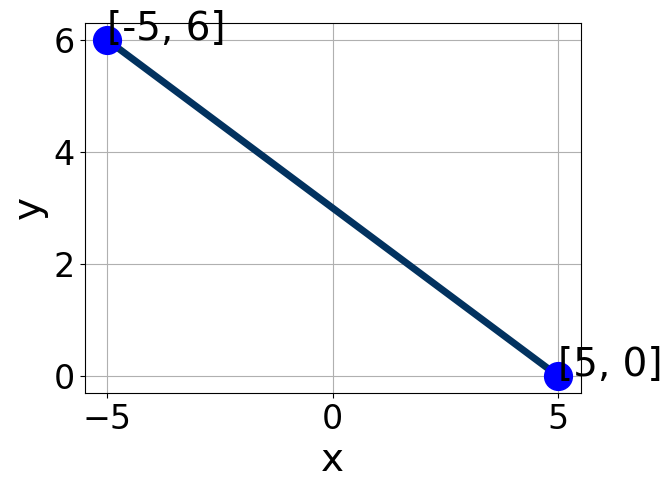
\includegraphics[width=0.5\textwidth]{../Figures/linearGraphToStandardC.png}
\end{center}
\begin{enumerate}[label=\Alph*.]
\item \( A \in [-1.1, 1], \hspace{3mm} B \in [-2.6, 0], \text{ and } \hspace{3mm} C \in [-6, -2] \)
\item \( A \in [2.9, 4.4], \hspace{3mm} B \in [-5.1, -4], \text{ and } \hspace{3mm} C \in [-20, -4] \)
\item \( A \in [-7.6, 0.5], \hspace{3mm} B \in [-5.1, -4], \text{ and } \hspace{3mm} C \in [-20, -4] \)
\item \( A \in [2.9, 4.4], \hspace{3mm} B \in [3.1, 6.3], \text{ and } \hspace{3mm} C \in [12, 19] \)
\item \( A \in [-1.1, 1], \hspace{3mm} B \in [0.5, 2.7], \text{ and } \hspace{3mm} C \in [3, 5] \)

\end{enumerate} }
\litem{
Find the equation of the line described below. Write the linear equation in the form $ y=mx+b $ and choose the intervals that contain $m$ and $b$.\[ \text{Perpendicular to } 5 x - 3 y = 15 \text{ and passing through the point } (5, 4). \]\begin{enumerate}[label=\Alph*.]
\item \( m \in [-0.67, -0.16] \hspace*{3mm} b \in [-7.6, -3.6] \)
\item \( m \in [-0.67, -0.16] \hspace*{3mm} b \in [6.5, 9.2] \)
\item \( m \in [-0.67, -0.16] \hspace*{3mm} b \in [-2, -0.9] \)
\item \( m \in [0.54, 1.76] \hspace*{3mm} b \in [0.2, 1.3] \)
\item \( m \in [-1.98, -1.35] \hspace*{3mm} b \in [6.5, 9.2] \)

\end{enumerate} }
\litem{
Solve the linear equation below. Then, choose the interval that contains the solution.\[ \frac{8x + 3}{7} - \frac{-3x + 8}{4} = \frac{7x + 4}{3} \]\begin{enumerate}[label=\Alph*.]
\item \( x \in [-21.5, -19.9] \)
\item \( x \in [1.5, 4.4] \)
\item \( x \in [-0.4, 1.7] \)
\item \( x \in [-7.1, -4.1] \)
\item \( \text{There are no real solutions.} \)

\end{enumerate} }
\litem{
Find the equation of the line described below. Write the linear equation in the form $ y=mx+b $ and choose the intervals that contain $m$ and $b$.\[ \text{Parallel to } 8 x + 9 y = 9 \text{ and passing through the point } (6, 4). \]\begin{enumerate}[label=\Alph*.]
\item \( m \in [-1, 0.3] \hspace*{3mm} b \in [-2.73, -1.89] \)
\item \( m \in [-1.3, -0.9] \hspace*{3mm} b \in [9.04, 9.97] \)
\item \( m \in [-0.3, 2.8] \hspace*{3mm} b \in [-1.84, -0.93] \)
\item \( m \in [-1, 0.3] \hspace*{3mm} b \in [-10.03, -8.99] \)
\item \( m \in [-1, 0.3] \hspace*{3mm} b \in [9.04, 9.97] \)

\end{enumerate} }
\litem{
Solve the equation below. Then, choose the interval that contains the solution.\[ -13(-16x -2) = -9(10x + 5) \]\begin{enumerate}[label=\Alph*.]
\item \( x \in [0.1, 0.21] \)
\item \( x \in [0.03, 0.14] \)
\item \( x \in [-0.26, -0.15] \)
\item \( x \in [-0.18, 0] \)
\item \( \text{There are no real solutions.} \)

\end{enumerate} }
\litem{
First, find the equation of the line containing the two points below. Then, write the equation in the form $ y=mx+b $ and choose the intervals that contain $m$ and $b$.\[ (7, -2) \text{ and } (-9, 3) \]\begin{enumerate}[label=\Alph*.]
\item \( m \in [-0.44, 0.04] \hspace*{3mm} b \in [-0.1, 1.7] \)
\item \( m \in [0.18, 0.4] \hspace*{3mm} b \in [4.48, 6.93] \)
\item \( m \in [-0.44, 0.04] \hspace*{3mm} b \in [-1.68, -0.09] \)
\item \( m \in [-0.44, 0.04] \hspace*{3mm} b \in [11.59, 12.01] \)
\item \( m \in [-0.44, 0.04] \hspace*{3mm} b \in [-9.78, -8.62] \)

\end{enumerate} }
\litem{
Write the equation of the line in the graph below in Standard Form $Ax+By=C$. Then, choose the intervals that contain $A, B, \text{ and } C$.
\begin{center}
    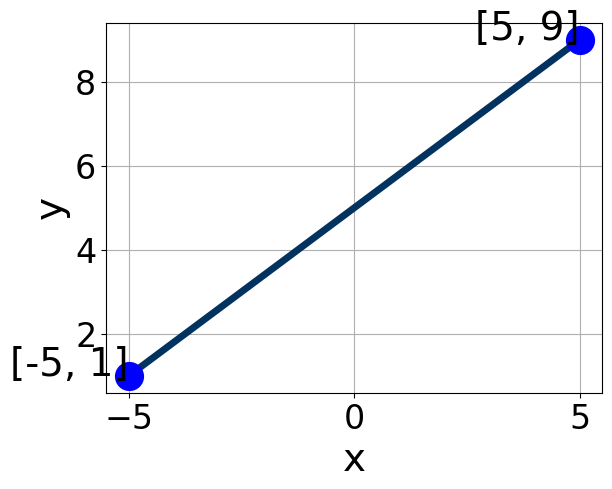
\includegraphics[width=0.5\textwidth]{../Figures/linearGraphToStandardCopyC.png}
\end{center}
\begin{enumerate}[label=\Alph*.]
\item \( A \in [-5.1, -3.9], \hspace{3mm} B \in [3.46, 5.47], \text{ and } \hspace{3mm} C \in [24, 29] \)
\item \( A \in [-3.8, 1.1], \hspace{3mm} B \in [-2.36, -0.99], \text{ and } \hspace{3mm} C \in [-6, -4] \)
\item \( A \in [-3.8, 1.1], \hspace{3mm} B \in [0, 1.29], \text{ and } \hspace{3mm} C \in [3, 7] \)
\item \( A \in [2.9, 7.6], \hspace{3mm} B \in [-5.22, -4.47], \text{ and } \hspace{3mm} C \in [-26, -17] \)
\item \( A \in [2.9, 7.6], \hspace{3mm} B \in [3.46, 5.47], \text{ and } \hspace{3mm} C \in [24, 29] \)

\end{enumerate} }
\litem{
Solve the linear equation below. Then, choose the interval that contains the solution.\[ \frac{-3x + 5}{2} - \frac{-6x + 9}{4} = \frac{-4x + 6}{5} \]\begin{enumerate}[label=\Alph*.]
\item \( x \in [0.2, 1.4] \)
\item \( x \in [10.7, 13.8] \)
\item \( x \in [-0.7, 0.2] \)
\item \( x \in [-5.1, -3.7] \)
\item \( \text{There are no real solutions.} \)

\end{enumerate} }
\end{enumerate}

\end{document}